\section{Appendix}

\subsection{DISCLAIMER}
\label{apdx:disclaimer}
The content presented in this article is intended for general informational purposes only and should not be construed as legal advice. Any views, opinions, findings, conclusions, or recommendations expressed in this material are the sole responsibility of the author(s) and do not represent the perspectives of any organization or entity.

\subsection{Additional Figure and Table}
\label{apdx:A}

Figure~\ref{fig:flowchart} illustrates the flowchart for minimizing license conflicts in a ML project.
Table~\ref{tab:list} lists the licenses supported by ModelGo.
Table~\ref{tab:works} shows the specifications of the involved data sources and models in the case studies.
Table~\ref{tab:stats} presents statistical data related to licenses and their corresponding count of works on Huggingface.
Table~\ref{tab:MLP} displays the summary of licensing details for ML projects with over 1K likes on Huggingface (\url{https://huggingface.co/}, projects in same series but different versions are omitted).

\begin{figure}[H]
  \centering
  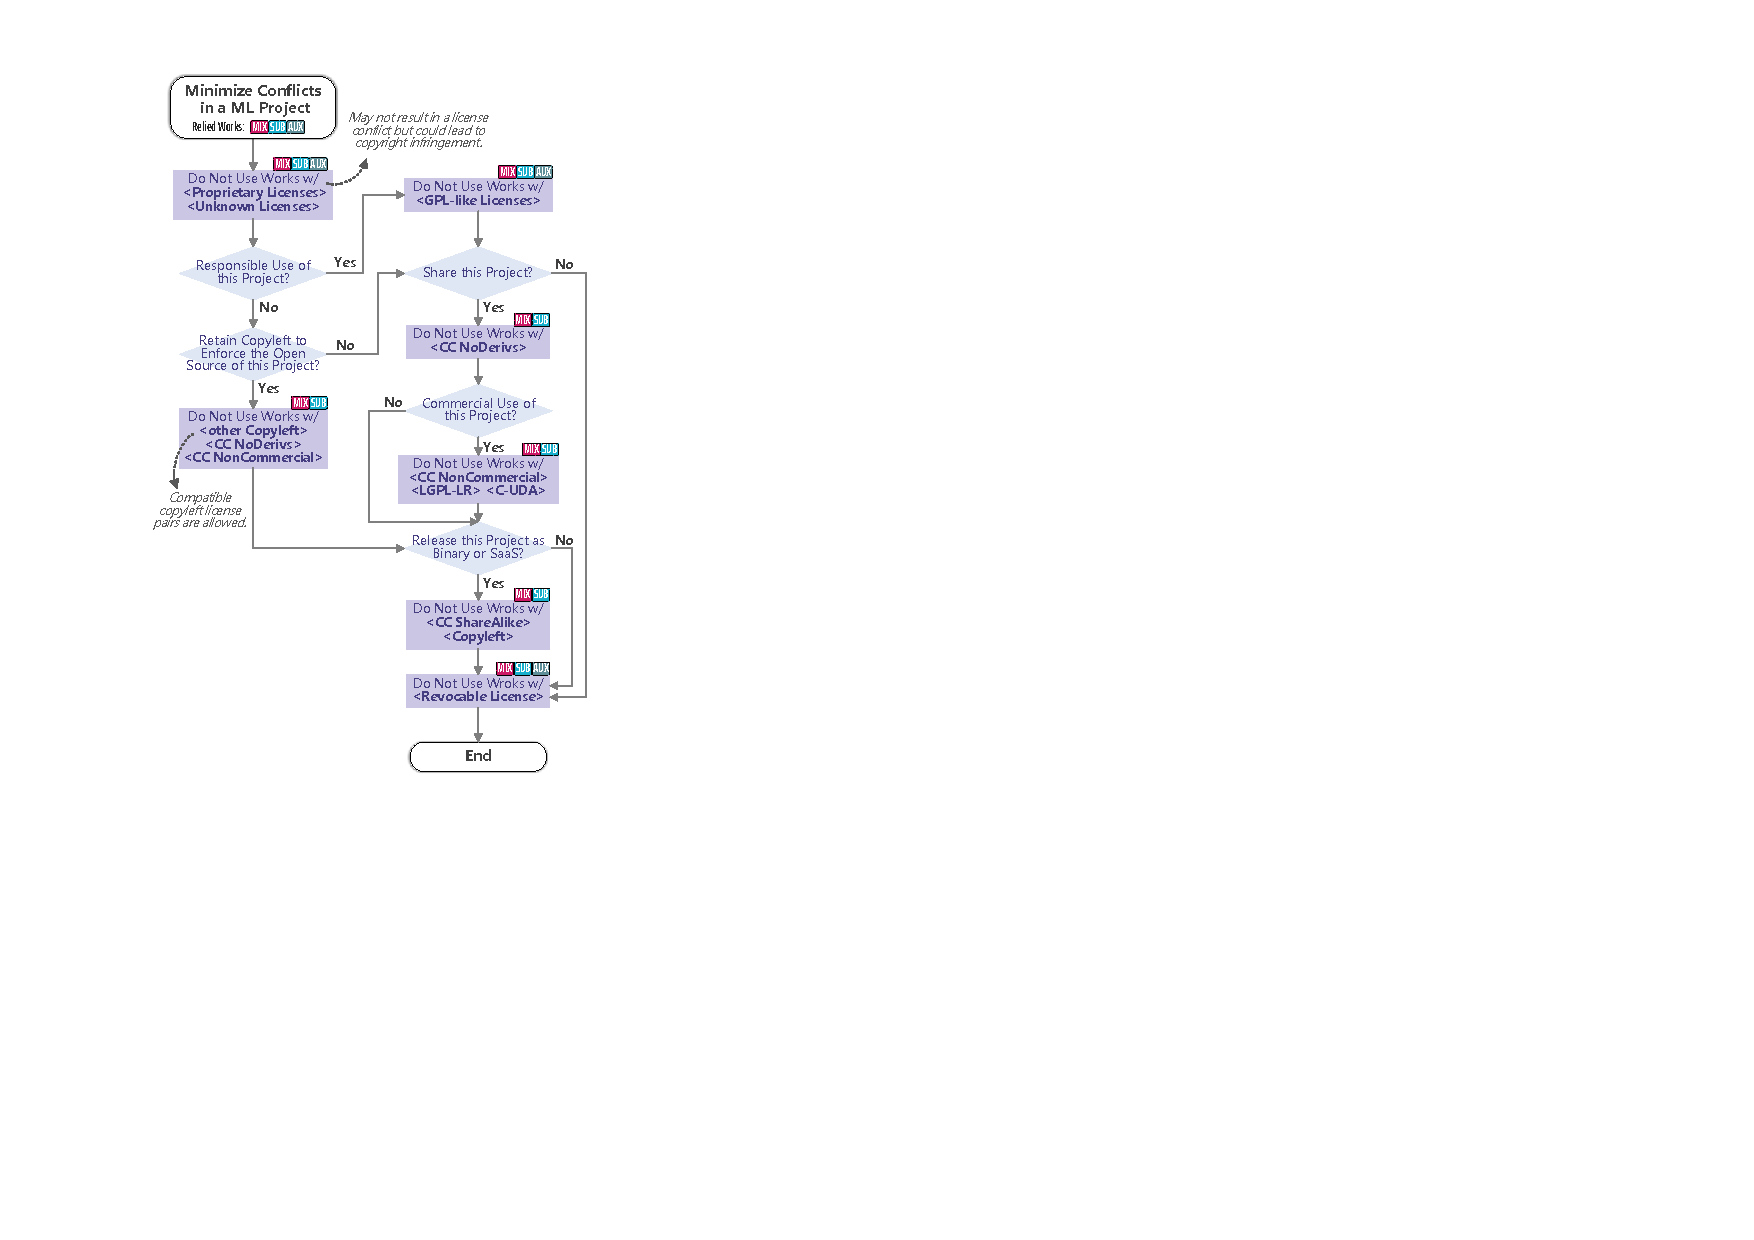
\includegraphics[scale=1]{fig/flowchart.pdf}
  \caption{Flowchart for minimizing license conflicts in ML projects.}
  \Description{}
  \label{fig:flowchart}
\end{figure}

\clearpage

\begin{table}[h]
  \caption{List of licenses (represented by SPDX short IDs) supported by ModelGo, covering over 96\% of licensed models and datasets on Huggingface.}
  %\vspace{-3mm}
  \scriptsize
  \label{tab:list}
  \begin{tabular}{|p{2.45cm}|p{2.45cm}|p{2.45cm}|}
  \hline
  \rowcolor[gray]{.8}
  \textbf{OSS License} (99.8\%) & \textbf{Content License} (96.6\%) & \textbf{AI Model License} (98.2\%)\\ \hline
  Apache-2.0, Unlicense, MIT, AFL-3.0, GPL-3.0, AGPL-3.0, LGPL-3.0, LGPL-2.1, BSD-3-Clause, BSD-3-Clause-Clear, BSD-2-Clause, Artistic-2.0, WTFPL-2.0, OSL-3.0, ECL-2.0
  &
  CC0-1.0, CC-BY-4.0, CC-BY-SA-4.0, CC-BY-NC-4.0, CC-BY-ND-4.0, CC-BY-NC-ND-4.0, CC-BY-NC-SA-4.0, PDDL, C-UDA, LGPL-LR, GFDL
  & 
  OpenRAIL++, CreativeML-OpenRAIL-M, BigScience-BLOOM-RAIL-1.0, Llama2, OPT-175B, SEER
  \\ \hline

  \end{tabular}
  %\vspace{-2mm}
\end{table}

\begin{table}[h]
  \caption{Specifications of AI components used in case studies, which include \textcolor{Copyleft}{Copyleft License}, \textcolor{Permissive}{Permissive License}, \textcolor{Public}{Public Domain License} and Non-Public License.}
  \vspace{-1mm}
  \footnotesize
  \label{tab:works}
  \begin{tabular}{|p{1.6cm}|p{3cm}|p{0.6cm}|p{1.7cm}|}
      \hline
      \rowcolor[gray]{.8}
      \textbf{Work Name} & \textbf{License Name} & \textbf{Type} & \textbf{Modality/Usage}  \\ \hline
      Wikipedia & \textcolor{Copyleft}{CC-BY-SA-4.0} & \multirow{15}{*}{Data} & \multirow{6}{*}{Text}   \\ \cline{1-2}
      StackExchange & \textcolor{Copyleft}{CC-BY-SA-4.0}  &  &    \\ \cline{1-2}
      FreeLaw & CC-BY-ND-4.0 &  &   \\ \cline{1-2}
      arXiv & \textcolor{Copyleft}{CC-BY-NC-SA-4.0} &  &   \\ \cline{1-2}
      PubMed & \textcolor{Copyleft}{CC-BY-NC-SA-4.0} &  &    \\ \cline{1-2}
      Deep-sequoia & CC-BY-NC-ND-4.0 &  &   \\ \cline{1-2} \cline{4-4}

      Midjourney Gen & CC-BY-NC-ND-4.0 &  & \multirow{6}{*}{Image}  \\ \cline{1-2}
      Flickr & \textcolor{Copyleft}{CC-BY-NC-SA-4.0} &  &   \\ \cline{1-2}
      StockSnap & \textcolor{Public}{CC0-1.0} &  &   \\ \cline{1-2}
      Wikimedia & \textcolor{Copyleft}{CC-BY-SA-4.0} &  &   \\ \cline{1-2}
      OpenClipart & \textcolor{Public}{CC0-1.0} &  &   \\ \cline{1-2} \cline{4-4}
      
      ccMixter & \textcolor{Permissive}{CC-BY-NC-4.0} & & \multirow{2}{*}{Voice}  \\ \cline{1-2}
      Jamendo & CC-BY-NC-ND-4.0 &  &   \\ \cline{1-2} \cline{4-4}
      
      Thingverse & \textcolor{Copyleft}{CC-BY-NC-SA-4.0} &  & 3D model  \\ \cline{1-2} \cline{4-4}

      Vimeo & CC-BY-NC-ND-4.0 &  & Video  \\ \hline

      Baize & \textcolor{Copyleft}{GPL-3.0} & \multirow{11}{*}{Model} & \multirow{4}{*}{Text Generation}   \\ \cline{1-2}
      BLOOM & \textcolor{Permissive}{BigScience-BLOOM-RAIL-1.0} & &   \\ \cline{1-2}
      Llama2 & \textcolor{Permissive}{Llama2 Community License} & &   \\ \cline{1-2}
      BigTranslate & \textcolor{Copyleft}{GPL-3.0} & &   \\ \cline{1-2} \cline{4-4}

      BERT & \textcolor{Permissive}{Apache-2.0} &  & Fill-Mask   \\ \cline{1-2} \cline{4-4}

      Stable Diffusion & \textcolor{Permissive}{CreativeML-OpenRAIL-M} & & Text to Image  \\ \cline{1-2} \cline{4-4}

      MaskFormer & \textcolor{Permissive}{CC-BY-NC-4.0} & & Image  \\ \cline{1-2}
      DETR & \textcolor{Permissive}{Apache-2.0} & & Segmentation \\ \cline{1-2} \cline{4-4}

      Whisper & \textcolor{Permissive}{MIT} & & Voice to Text  \\ \cline{1-2} \cline{4-4}

      X-Clip & \textcolor{Permissive}{MIT} & & Video to Text  \\ \cline{1-2} \cline{4-4}

      I2VGen-XL & CC-BY-NC-ND-4.0 & & Image to Video  \\ \hline

      \end{tabular}
\end{table}

\begin{table}[h]
  \caption{List of Huggingface supported licenses and work count, with ModelGo supported licenses highlighted in BOLD. Note that many works do not explicitly indicate their license version. (Accessed on October 11, 2023). }
  \scriptsize
  \label{tab:stats}
  \begin{tabular}{|ll||ll|}
  \hline
  \rowcolor[gray]{.8} 
  \multicolumn{2}{|c||}{Model (Total Work: 355,150)}     & \multicolumn{2}{c|}{Dataset (Total Work: 69,277)}   \\ \hline
  \rowcolor[gray]{.9} 
  \multicolumn{1}{|l|}{License Name} & Count & \multicolumn{1}{l|}{License Name} & Count \\ \hline
  \multicolumn{1}{|l|}{\textbf{Apache-2.0}} & 46,758 & \multicolumn{1}{l|}{MIT} & 5,415 \\ \hline
  \multicolumn{1}{|l|}{\textbf{MIT}} & 21,365 & \multicolumn{1}{l|}{Apache-2.0} & 3,026 \\ \hline %3020+6
  \multicolumn{1}{|l|}{OpenRAIL} & 17,760 & \multicolumn{1}{l|}{OpenRAIL} & 1,639 \\ \hline
  \multicolumn{1}{|l|}{\textbf{CreativeML-OpenRAIL-M}} & 12,059 & \multicolumn{1}{l|}{\textbf{CC-BY-4.0}} & 1,355 \\ \hline
  \multicolumn{1}{|l|}{other} & 6,521 & \multicolumn{1}{l|}{other} & 1,257 \\ \hline
  \multicolumn{1}{|l|}{CC-BY-NC-4.0} & 2,867 & \multicolumn{1}{l|}{\textbf{CC-BY-SA-4.0}} & 609 \\ \hline
  \multicolumn{1}{|l|}{CC-BY-4.0} & 2,676 & \multicolumn{1}{l|}{AFL-3.0} & 515 \\ \hline
  \multicolumn{1}{|l|}{\textbf{AFL-3.0}} & 2,111 & \multicolumn{1}{l|}{CC} & 444 \\ \hline
  \multicolumn{1}{|l|}{\textbf{Llama2}} & 1,776 & \multicolumn{1}{l|}{\textbf{CC0-1.0}} & 435 \\ \hline
  \multicolumn{1}{|l|}{CC-BY-NC-SA-4.0} & 1,312 & \multicolumn{1}{l|}{\textbf{CC-BY-NC-4.0}} & 385 \\ \hline
  \multicolumn{1}{|l|}{\textbf{GPL-3.0}} & 1,080 & \multicolumn{1}{l|}{\textbf{CC-BY-NC-SA-4.0}} & 378 \\ \hline
  \multicolumn{1}{|l|}{CC-BY-SA-4.0} & 959 & \multicolumn{1}{l|}{CC-BY-SA-3.0} & 377 \\ \hline
  \multicolumn{1}{|l|}{\textbf{OpenRAIL++}} & 667 & \multicolumn{1}{l|}{CreativeML-OpenRAIL-M} & 290 \\ \hline
  \multicolumn{1}{|l|}{CC} & 625 & \multicolumn{1}{l|}{GPL-3.0} & 266 \\  \hline
  \multicolumn{1}{|l|}{\textbf{BigScience-OpenAI-M}} & 596 & \multicolumn{1}{l|}{\textbf{CC-BY-NC-ND-4.0}} & 190 \\ \hline
  \multicolumn{1}{|l|}{\textbf{Artistic-2.0}} & 579 & \multicolumn{1}{l|}{BigScience-OpenRAIL-M} & 114 \\ \hline
  \multicolumn{1}{|l|}{\textbf{BSD-3-Clause}} & 525 & \multicolumn{1}{l|}{CC-BY-3.0} & 94 \\ \hline
  \multicolumn{1}{|l|}{\textbf{BigScience-BLOOM-RAIL-1.0}} & 422 & \multicolumn{1}{l|}{CC-BY-2.0} & 91 \\ \hline
  \multicolumn{1}{|l|}{\textbf{WTFPL}} & 331 & \multicolumn{1}{l|}{Artistic-2.0} & 91 \\ \hline
  \multicolumn{1}{|l|}{CC-BY-SA-3.0} & 288 & \multicolumn{1}{l|}{ODC-by} & 80 \\ \hline
  \multicolumn{1}{|l|}{CC0-1.0} & 270 & \multicolumn{1}{l|}{WTFPL} & 80 \\ \hline
  \multicolumn{1}{|l|}{\textbf{BigCode-OpenRAIL-M}} & 251 & \multicolumn{1}{l|}{Unlicense} & 68 \\ \hline
  \multicolumn{1}{|l|}{\textbf{AGPL-3.0}} & 237 & \multicolumn{1}{l|}{Llama2} & 63 \\ \hline
  \multicolumn{1}{|l|}{\textbf{Unlicense}} & 199 & \multicolumn{1}{l|}{BSD} & 62 \\ \hline
  \multicolumn{1}{|l|}{CC-BY-NC-ND-4.0} & 194 & \multicolumn{1}{l|}{GPL} & 54 \\ \hline
  \multicolumn{1}{|l|}{GPL} & 173 & \multicolumn{1}{l|}{\textbf{C-UDA}} & 49 \\ \hline
  \multicolumn{1}{|l|}{BSD} & 155 & \multicolumn{1}{l|}{AGPL-3.0} & 46 \\ \hline
  \multicolumn{1}{|l|}{CC-BY-3.0} & 104 & \multicolumn{1}{l|}{CC-BY-NC-SA-3.0} & 38 \\ \hline
  \multicolumn{1}{|l|}{GPL-2.0} & 84 & \multicolumn{1}{l|}{ODBL} & 35 \\ \hline
  \multicolumn{1}{|l|}{CC-BY-2.0} & 80 & \multicolumn{1}{l|}{\textbf{GFDL}} & 34 \\ \hline
  \multicolumn{1}{|l|}{BSL-1.0} & 75 & \multicolumn{1}{l|}{BSD-3-Clause} & 34 \\ \hline
  \multicolumn{1}{|l|}{\textbf{BSD-2-Clause}} & 74 & \multicolumn{1}{l|}{\textbf{CC-BY-ND-4.0}} & 32 \\ \hline
  \multicolumn{1}{|l|}{\textbf{LGPL-3.0}} & 65 & \multicolumn{1}{l|}{CC-BY-NC-3.0} & 28 \\ \hline
  \multicolumn{1}{|l|}{C-UDA} & 57 & \multicolumn{1}{l|}{BigScience-BLOOM-RAIL-1.0} & 28 \\ \hline
  \multicolumn{1}{|l|}{CC-BY-NC-2.0} & 48 & \multicolumn{1}{l|}{GPL-2.0} & 26 \\ \hline
  \multicolumn{1}{|l|}{CC-BY-NC-3.0} & 45 & \multicolumn{1}{l|}{OpenRAIL++} & 24 \\ \hline
  \multicolumn{1}{|l|}{\textbf{OSL-3.0}} & 44 & \multicolumn{1}{l|}{CC-BY-NC-2.0} & 21 \\ \hline
  \multicolumn{1}{|l|}{\textbf{ECL-2.0}} & 35 & \multicolumn{1}{l|}{BigCode-OpenRAIL-M} & 20 \\ \hline
  \multicolumn{1}{|l|}{PDDL} & 35 & \multicolumn{1}{l|}{\textbf{PDDL}} & 20 \\ \hline
  \multicolumn{1}{|l|}{\textbf{BSD-3-Clause-Clear}} & 28 & \multicolumn{1}{l|}{BSD-2-Clause} & 16 \\ \hline
  \multicolumn{1}{|l|}{CC-BY-ND-4.0} & 27 & \multicolumn{1}{l|}{LGPL-3.0} & 15 \\ \hline
  \multicolumn{1}{|l|}{GFDL} & 26 & \multicolumn{1}{l|}{CDLA-Sharing-1.0} & 14 \\ \hline
  \multicolumn{1}{|l|}{Ms-PL} & 26 & \multicolumn{1}{l|}{CC-BY-2.5} & 12 \\ \hline
  \multicolumn{1}{|l|}{Zlib} & 25 & \multicolumn{1}{l|}{Ms-PL} & 11 \\ \hline
  \multicolumn{1}{|l|}{LGPL} & 21 & \multicolumn{1}{l|}{CDLA-Permissive-2.0} & 11 \\ \hline
  \multicolumn{1}{|l|}{DeepFloyd-IF-License} & 19 & \multicolumn{1}{l|}{CC-BY-NC-SA-2.0} & 10 \\ \hline
  \multicolumn{1}{|l|}{CC-BY-NC-SA-3.0} & 19 & \multicolumn{1}{l|}{MPL-2.0} & 10 \\ \hline
  \multicolumn{1}{|l|}{LGPL-LR} & 17 & \multicolumn{1}{l|}{EUPL-1.1} & 10 \\ \hline
  \multicolumn{1}{|l|}{MPL-2.0} & 16 & \multicolumn{1}{l|}{CC-BY-NC-ND-3.0} & 10 \\ \hline
  \multicolumn{1}{|l|}{ISC} & 15 & \multicolumn{1}{l|}{BSL-1.0} & 10 \\ \hline
  \multicolumn{1}{|l|}{CC-BY-NC-SA-2.0} & 15 & \multicolumn{1}{l|}{BSD-3-Clause-Clear} & 8 \\ \hline
  \multicolumn{1}{|l|}{ODBL} & 15 & \multicolumn{1}{l|}{LGPL} & 6 \\ \hline
  \multicolumn{1}{|l|}{CC-BY-2.0} & 14 & \multicolumn{1}{l|}{ECL-2.0} & 6 \\ \hline
  \multicolumn{1}{|l|}{CC-BY-NC-ND-3.0} & 14 & \multicolumn{1}{l|}{OSL-3.0} & 5 \\ \hline
  \multicolumn{1}{|l|}{ODB-by} & 13 & \multicolumn{1}{l|}{ISC} & 5 \\ \hline
  \multicolumn{1}{|l|}{NCSA} & 9 & \multicolumn{1}{l|}{\textbf{LGPL-LR}} & 4 \\ \hline
  \multicolumn{1}{|l|}{EPL-2.0} & 9 & \multicolumn{1}{l|}{PostgreSQL} & 3 \\ \hline
  \multicolumn{1}{|l|}{EUPL-1.1} & 9 & \multicolumn{1}{l|}{Zlib} & 3 \\ \hline
  \multicolumn{1}{|l|}{CDLA-Sharing-1.0} & 7 & \multicolumn{1}{l|}{EPL-2.0} & 2 \\ \hline
  \multicolumn{1}{|l|}{\textbf{LGPL-2.1}} & 6 & \multicolumn{1}{l|}{OFL-1.1} & 2 \\ \hline
  \multicolumn{1}{|l|}{PostgreSQL} & 5 & \multicolumn{1}{l|}{LGPL-2.1} & 1 \\ \hline
  \multicolumn{1}{|l|}{LPPL-1.3c} & 5 & \multicolumn{1}{l|}{CDLA-Permissive-1.0} & 1 \\ \hline
  \multicolumn{1}{|l|}{EPL-1.0} & 4 & \multicolumn{1}{l|}{CC-BY-2.0} & 1 \\ \hline
  \multicolumn{1}{|l|}{OFL-1.1} & 3 & \multicolumn{1}{l|}{NCSA} & 1 \\ \hline
  \multicolumn{1}{|l|}{TII-Falcon-LLM} & 2 & \multicolumn{1}{l|}{DeepFloyd-IF-License} & 1 \\ \hline
  \multicolumn{1}{|l|}{CDLA-Permissive-2.0} & 2 & \multicolumn{1}{l|}{EPL-1.0} & 1 \\ \hline
  \multicolumn{1}{|l|}{CDLA-Permissive-1.0} & 2 & \multicolumn{1}{l|}{LPPL-1.3c} & 1 \\ \hline
  \end{tabular}
\end{table}

\clearpage

\begin{table*}[h]
  \caption{Summary of licensing details for ML projects with over 1K likes on Huggingface (Accessed on October 11, 2023). }
  \footnotesize
  \label{tab:MLP}
  \begin{tabular}{|p{2.1cm}|p{1.6cm}|p{2cm}|p{2.75cm}|p{3cm}|p{1.7cm}|p{2cm}|}
      \hline
      \rowcolor[gray]{.8}
      \textbf{ML Project} & \textbf{Task} & \textbf{Data License} & \textbf{Software License} & \textbf{Model License} & \textbf{Dataset} & \textbf{Risk Resource} \\ \hline
      
      Stable Diffusion v1-5 & Text to Image & CC-BY-4.0 & CreativeML-OpenRAIL-M & CreativeML-OpenRAIL-M & LAION-5B & Common Crawl \\ \hline
      
      BLOOM & Text Generation & \textit{Mixture} & \textit{Unknown} & BigScience-BLOOM-RAIL-1.0 & \textit{Crowdsourced} & Common Crawl, \newline Wikipedia, etc. \\ \hline

      OrangeMixs & Text to Image & \textit{Mixture} & \textit{Unknown} & CreativeML-OpenRAIL-M & \textit{Crowdsourced} & Danbooru \\ \hline

      ControlNet & Text to Image &  \textit{Unknown} & Apache-2.0 & OpenRAIL & \textit{Unknown} & n/a \\ \hline

      Openjourney & Text to Image &  CC-BY-NC-4.0 & \textit{Unknown} & CreativeML-OpenRAIL-M & Midjourney Gen & Midjourney Gen \\ \hline

      ChatGLM-6B & Text Generation &  \textit{Mixture} & Apache-2.0 & \textit{Custom} & the Pile, Wudao, \newline \textit{Crowdsourced} & PubMed,  Wikipedia, \newline arXiv, GitHub, etc. \\ \hline

      Llama2 & Text Generation &  \textit{Unknown} & Llama2 Community License & Llama2 Community License & \textit{Unknown} & n/a \\ \hline

      StarCoder & Text Generation &  \textit{Mixture} & Apache-2.0 & BigCode-OpenRAIL-M & The Stack & none \\ \hline

      Falcon-40B & Text Generation & ODC-By & Apache-2.0 & Apache-2.0 & RefinedWeb & Wikipedia, Reddit, \newline StackOverflow, etc. \\ \hline

      Waifu Diffusion & Text to Image & \textit{Mixture} & \textit{Unknown} & CreativeML-OpenRAIL-M & \textit{Unknown} & n/a \\ \hline

      Dolly-v2-12B & Text Generation & CC-BY-SA-3.0\&4.0 & MIT & MIT & databricks-dolly\newline-15k, the Pile & PubMed,  Wikipedia, \newline arXiv, GitHub, etc. \\ \hline

      Dreamlike Photoreal & Text to Image & \textit{Unknown} & \textit{Unknown} & \textit{Modified} CreativeML-\newline OpenRAIL-M & \textit{Unknown} & n/a \\ \hline

      Counterfeit & Text to Image & \textit{Unknow} & \textit{Unknown} & CreativeML-OpenRAIL-M & \textit{Unknown} & n/a \\ \hline

      GPT-2 & Text Generation & \textit{Mixture} & \textit{Modified} MIT & \textit{Modified} MIT & \textit{Crowdsourced} & WordPress, GitHub, \newline wikiHow, IMDb, etc. \\ \hline

      GPT-J-6B & Text Generation & \textit{Mixture} & Apache-2.0 & Apache-2.0 & the Pile & PubMed,  Wikipedia, \newline arXiv, GitHub, etc. \\ \hline

      LLaMA-7B & Text Generation & \textit{Mixture} & \textit{Custom} & \textit{Custom} & \textit{Crowdsourced} & GitHub, arXiv, etc. \\ \hline

      BERT & Fill Mask & \textit{Mixture} & Apache-2.0 & Apache-2.0 & Book Corpus, \newline Wikipedia (en) & Wikipedia (en) \\ \hline

      Whisper & ASR & \textit{Unknown} & MIT & MIT & \textit{Unknown} & n/a \\ \hline

      MPT & Text Generation & \textit{Mixture} & Apache-2.0 & Apache-2.0 & \textit{Crowdsourced} & Common Crawl, \newline Wikipedia, etc. \\ \hline

      Mistral-7B & Text Generation & \textit{Unknow} & Apache-2.0 & Apache-2.0 & \textit{Unknow} & n/a \\ \hline
  
  % <TOTAL>
  % Data License: All Permissive(2); Risk of Copyleft/Proprietary(11); Custom/Modified(0); Unknown(6);
  % Software License: Permissive(11); Risk of Copyleft/Proprietary(n/a); Custom/Modified(2); Unknown(6);
  % Model License: Permissive(15); Risk of Copyleft/Proprietary(n/a); Custom/Modified(4); Unknown(0);

  \end{tabular}
\end{table*}